% !TeX root = ../tfg.tex
% !TeX encoding = utf8
\chapter{¿Qué es un juego?} \label{cap1}

% --- Epígrafe alineado a la derecha ---

\begin{flushright}
\itshape
``Hace tiempo que ha ido cuajando en mí la convicción de que la cultura humana brota del juego -como juego- y en él se desarrolla. \\
El juego es más viejo que la cultura; pues, por mucho que estrechemos el concepto de ésta, presupone siempre una sociedad humana, y los animales no han esperado a que el hombre les enseñara a jugar. ''\\[1ex]
\hrulefill\\[-0.5ex]
\small Johan Huizinga, \textit{Homo Ludens} (1938) \cite{huizinga1938}
\end{flushright}

\vspace{2em}

Para entender lo que es un juego, en primera instancia, debemos definir el concepto con el fin de concretar a qué nos referimos al hablar de uno. Tras esto, abordaremos el desarrollo de un juego y el diseño de un agente capaz de jugarlo.

En este capítulo se analiza la definición de ``juego`` desde el punto de vista de la Teoría de Juegos. A partir de esta definición, se propone una clasificación y se presentan varias formas de representación formal.
Por último, se ofrece una definición del concepto de ``juego`` desde la perspectiva del diseño, a pesar de la dificultad que conlleva dicha tarea.

\section{Teoría de Juegos}

Esta sección se basa en los contenidos de \textit{Teoría de Juegos} (Cerdá, Pérez y Jimeno, 2004) \cite{TeoriaDeJuegosCJP}.

El concepto de juego en el ámbito matemático está estrechamente relacionado con la Teoría de Juegos, disciplina que surge en 1944 con la publicación de \textit{Game Theory and Economic Behavior} \cite{VonNeumannMorgenstern1944}, de Von Neumann y Morgenstern. Aunque existen trabajos anteriores que tratan ideas similares, no será hasta esta obra cuando se asienten las bases de la Teoría de Juegos moderna, centrada en el análisis y la resolución de conflictos estratégicos.

Aunque la Teoría de Juegos no se desarrolló con el propósito de estudiar la faceta lúdica de los juegos, sino su componente estratégico y sus aplicaciones al análisis de sistemas complejos en economía, biología o sociología, en capítulos posteriores abordaremos precisamente esta dimensión lúdica, desde la perspectiva del diseño de juegos.

\subsection{Definición}
Entendemos ``juego`` como una situación en la que cada participante busca lograr el mejor resultado posible (maximizar su utilidad), sabiendo que el resultado no depende únicamente de sus propias decisiones, sino también de las decisiones de los demás. Dentro del marco de la Teoría de Juegos, nos centraremos en el análisis de la interacción estratégica entre los jugadores.

De este modo, la Teoría de Juegos puede considerarse como una teoría de la decisión interactiva, diferenciada de la teoría de la decisión individual. 

Para este primer acercamiento, es conveniente explicitar algunos conceptos básicos: %\cite{TeoriaDeJuegosCJP}

\begin{itemize}
    \item \textbf{Jugadores}: Participantes del juego que toman decisiones buscando maximizar su utilidad. Pueden ser dos o más.
    \item \textbf{Acciones}: Conjunto de decisiones disponibles para un jugador en un momento determinado.
    \item \textbf{Resultados}: Conjunto de estados en los que se da por finalizado el juego.
    \item \textbf{Pagos}: Ganancias o pérdidas que recibe cada jugador al terminar la partida. Estos dependen del resultado obtenido y nos dan la utilidad que cada jugador va a asociar a ese estado.
    \item \textbf{Estrategias}: Plan completo de acción que sigue un jugador al participar en el juego. Podemos agrupar las estrategias en perfiles de estrategias seguidos por cada jugador.
\end{itemize}

\subsection{Tipos de juegos}
La primera gran distinción que se puede hacer dentro del ámbito de los juegos es entre \textbf{cooperativos} y \textbf{no cooperativos}.

En los juegos \textbf{cooperativos}, los jugadores coordinan sus estrategias o establecen acuerdos para maximizar un beneficio conjunto. Por el contrario, en los \textbf{no cooperativos}, cada jugador toma decisiones de forma independiente, buscando su propio beneficio.

Este trabajo se centra en los juegos \textbf{no cooperativos}, ya que nos enfocamos en aquellos juegos en los que los jugadores están en enfrentamiento directo. Dentro de este ámbito, se distinguen cuatro categorías generales:

\begin{itemize}
\item \textbf{Juegos estáticos}: Los jugadores deciden simultáneamente, sin conocer las decisiones ajenas. 

\item \textbf{Juegos dinámicos}: Un jugador puede llegar a conocer las decisiones de otro participante antes de tomar su decisión. Usualmente, son juegos que pueden contar con turnos.

\item \textbf{Juegos con información completa}: Todos los jugadores conocen el estado completo del juego y, por tanto, de las posibles consecuencias de sus acciones.

\item \textbf{Juegos con información incompleta}: Al menos un jugador no conoce el estado completo del juego, impidiendo así la posibilidad de conocer las consecuencias de alguna acción.
\end{itemize}

\subsection{Representación formal}
Una vez expuesto qué es un juego, cuáles son sus elementos principales y su clasificación, se plantea a continuación cómo podemos representar uno de forma rigurosa. 
\newline

Pueden ser representados de manera \textbf{estratégica} o \textbf{extensiva}. En ambas se explicitan los jugadores, las acciones y los pagos. 

La \textbf{estratégica} utiliza una matriz que recoge todas las combinaciones posibles de acciones y los pagos asociados, permitiendo visualizar de manera compacta las estrategias disponibles para cada jugador.

La \textbf{extensiva}, en cambio, representa el juego mediante un árbol de decisiones que muestra de forma secuencial el desarrollo del mismo.

De manera general, se emplea la representación estratégica para juegos estáticos y la extensiva para los dinámicos.

Primero, se definen los siguientes elementos, que son comunes a ambas formas de representación:
\begin{itemize}
    \item \textbf{El conjunto de jugadores}, J. Podemos escribir $J=\{j_1,...,j_n\}$ para un juego con $n$ jugadores. 
        Por simplicidad en la notación, es conveniente que cada $j_i=i$ sea entero. Por tanto, un juego de $n$ jugadores quedaría como $J=\{1,2,...,n\}$.
    \item \textbf{Los conjuntos de acciones}. Cada jugador $i\in J$ tiene un conjunto de acciones $A_i$ posibles ante cada situación.
    \item \textbf{Los conjuntos de estrategias}. Cada jugador $i\in J$ tiene un conjunto de estrategias $S_i$. Las estrategias definen qué acciones debe tomar ese jugador ante una situación.
    \item \textbf{Los perfiles de estrategias}. Cada perfil $s=(s_1,...,s_n)$ es la n-upla que describe la estrategia seguida por cada uno de los $n$ jugadores. El perfil de estrategias nos da los posibles desarrollos del juego. 
    \item \textbf{Las funciones de pagos}. Habrá un pago para cada jugador $i\in J$ por jugar cada perfil de estrategias $s$, $\{u_i(s)\}_{i\in J}$.
    
\end{itemize}

Con todo esto presente, describimos el juego $G$ como:
 \begin{equation}
     G=\bigg{\{}J,\{S_i\}_{i\in J},\{u_i(s)\}_{i\in J}\bigg{\}}
 \end{equation}
 
\hfill \break

\textbf{Forma estratégica:}

 Para ver su representación en una matriz bidimensional, suponemos $J=\{1,2\}$.

 Si el jugador 1 tiene estrategias $(S_1={s_{11},s_{12},...,s_{1m}})$ y el jugador 2 tiene estrategias $(S_2={s_{21},s_{22},...,s_{2n}})$, la matriz de pagos es:
\[
\begin{array}{|c|c|c|c|c|}
    \hline
    & \multicolumn{4}{|c|}{\textbf{J2}} \\ \hline
    & s_{21} & s_{22} & \cdots & s_{2n} \\ \hline
    \multirow{4}{*}{\textbf{J1}} 
    & (u_1(s_{11},s_{21}),u_2(s_{11},s_{21})) & (u_1(s_{11},s_{22}),u_2(s_{11},s_{22})) & \cdots & (u_1(s_{11},s_{2n}),u_2(s_{11},s_{2n})) \\ \cline{2-5}
    & (u_1(s_{12},s_{21}),u_2(s_{12},s_{21})) & (u_1(s_{12},s_{22}),u_2(s_{12},s_{22})) & \cdots & (u_1(s_{12},s_{2n}),u_2(s_{12},s_{2n})) \\ \cline{2-5}
    & \vdots & \vdots & \ddots & \vdots \\ \cline{2-5}
    & (u_1(s_{1m},s_{21}),u_2(s_{1m},s_{21})) & (u_1(s_{1m},s_{22}),u_2(s_{1m},s_{22})) & \cdots & (u_1(s_{1m},s_{2n}),u_2(s_{1m},s_{2n})) \\
    \hline
\end{array}
\]

Cada celda corresponde al par de pagos $((u_1, u_2))$ resultante del perfil de estrategias escogido.

En el Capítulo 3 se exponen ejemplos concretos de juegos representados de forma estratégica como el dilema del prisionero \ref{prisionero} o piedra papel y tijeras \ref{piedra_papel_tijeras}.

\hfill \break.

\textbf{Forma extensiva:}
En la forma extensiva nos apoyamos en un árbol donde los jugadores toman decisiones y van ejecutando acciones sucesivamente. 

Veamos cómo sería un juego $G=\bigg{\{}\{1,2\},\{S_i\}_{i\in J},\{u_i(s)\}_{i\in J}\bigg{\}}$ donde las acciones posibles son $A_1=\{A,B\}$ para el J1 y $A_2=\{C,D,F,G\}$ para J2. Como no podemos representar todos los perfiles de estrategias, a continuación representamos uno donde:
\begin{itemize}
    \item J1 elige entre $A$ y $B$.
    \item Si elige $A$, entonces J2 elige entre $C$ y $D$.
    \item Si elige $B$, entonces J2 elige entre $E$ y $F$.

\end{itemize}

Al final de cada rama hay un vector de pagos $(u_1,u_2)$.

\[
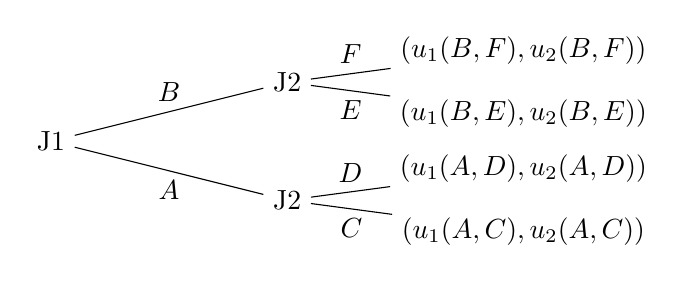
\begin{tikzpicture}[grow=right, level distance=30mm,
    level 2/.style={sibling distance=8mm}] % más distancia vertical en las hojas
\node {J1}
    child {
        node {J2}
            child { node {$(u_1(A,C),u_2(A,C))$} edge from parent node[below] {$C$}}
            child { node {$(u_1(A,D),u_2(A,D))$} edge from parent node[above] {$D$}}
            edge from parent node[below] {$A$}
    }
    child {
        node {J2}
            child { node {$(u_1(B,E),u_2(B,E))$} edge from parent node[below] {$E$}}
            child { node {$(u_1(B,F),u_2(B,F))$} edge from parent node[above] {$F$}}
            edge from parent node[above] {$B$}
    };
\end{tikzpicture}
\]

De esta forma, podemos representar las acciones de forma secuencial y los pagos a los que llega cada jugador.

En el Capítulo 3 se exponen ejemplos concretos de juegos representados de forma extensiva como el tres en raya \ref{tres_en_raya} o el ajedrez \ref{ajedrez}.

 
%Aunque vamos a detenernos en dar ejemplos de cada tipo de juego, es necesario definir dos juegos muy simples que nos ilustren ambos tipos de representación.



\section{Pero, ¿qué es realmente un juego?} \label{que_es_juego}
Definir qué es un juego puede parecer trivial a primera vista, pero se trata de una tarea sorprendentemente compleja y profundamente relevante para cualquier diseñador. La necesidad de una definición precisa no es meramente académica: no podemos aspirar a mejorar en la creación de juegos si no somos capaces de articular qué es lo que estamos diseñando. En este sentido, disponer de un vocabulario común y bien delimitado permite no solo comunicar ideas, sino también evaluar y criticar mecánicas, estructuras y experiencias lúdicas de manera rigurosa. \cite{costikyan2002}

A lo largo de la historia, distintos autores han intentado capturar la esencia del juego desde perspectivas diversas:

\subsection{Juegos como actividades culturales y sociales}

Joh Huizinga, en su influyente obra \textit{Homo Ludens} (1938) \cite{huizinga1938}, propone una definición amplia y abarcativa:

\begin{quote}
``El juego, en su aspecto formal, es una acción libre ejecutada \texttt{<<como sí>>} y sentida como situada fuera de la vida corriente, pero que, a pesar de todo, puede absorber por completo al jugador, sin que haya en ella ningún interés material ni se obtenga en ella provecho alguno, que se ejecuta dentro de un determinado tiempo y un determinado espacio, que se desarrolla en un orden sometido a reglas y que da origen a asociaciones que propenden a rodearse de misterio o a disfrazar para destacarse del mundo habitual.''
\end{quote}

Según Huizinga, el juego es:

\begin{itemize}
    \item Libre y voluntario.
    \item Desarrollado dentro de límites de tiempo y espacio.
    \item Regido por reglas.
    \item Sin finalidad práctica, es decir, un fin en sí mismo.
    \item Acompañado de tensión, alegría y separación de la vida ordinaria.
\end{itemize}

Si bien esta definición es profunda y culturalmente rica, resulta demasiado amplia para el contexto del diseño de videojuegos, ya que engloba prácticas como el teatro, rituales y otras formas de juego simbólico que no necesariamente comparten las propiedades interactivas y mecánicas de los videojuegos modernos.

\subsection{Juegos como superación de obstáculos}

Bernard Suits, en \emph{The Grasshopper: Games, Life and Utopia} (1978) \cite{suits1978}, propone un enfoque más formal y filosófico:

\begin{quote}
``Playing a game is the voluntary attempt to overcome unnecessary obstacles.''
\end{quote} 


Suits desarrolla esta definición mediante cuatro componentes fundamentales:

\begin{enumerate}
    \item Una actividad en la que los participantes intentan alcanzar un estado meta (\textit{prelusory goal}).
    \item Usando solo los medios permitidos por las reglas (\textit{lusory means}).
    \item Donde las reglas prohíben usar medios más eficaces para alcanzar la meta.
    \item Y los jugadores aceptan estas reglas precisamente porque hacen posible la actividad (\textit{lusory attitude}).
\end{enumerate}

Aunque la definición de Suits se ajusta bien a juegos de mesa o deportivos, se queda corta para capturar las dinámicas interactivas y experienciales de los videojuegos modernos, donde elementos como la narrativa, la exploración o la elección del jugador son fundamentales y no siempre encajan en la idea de ``obstáculos innecesarios''.

Esta definición resultó especialmente útil para el filósofo C. Thi Nguyen en su obra \textit{Games: Agency As Art (Thinking Art)}, donde reflexiona sobre los juegos como un medio artístico que explora la agencia humana. Nguyen reconoce desde el inicio la dificultad de proporcionar una definición satisfactoria de este fenómeno. Apoyándose en la concepción de Suits, introduce el término \textit{suitsian game} para referirse a aquellos juegos que poseen reglas formales y objetivos definidos, diferenciándolos del juego libre o abierto a la improvisación.

\subsection{La necesidad de un vocabulario para diseñar}

El artículo \textit{I Have No Words and I Must Design} \cite{costikyan2002} de Greg Costikyan aborda de manera explícita la dificultad de definir juegos y la importancia de contar con un vocabulario compartido en el diseño. Costikyan propone una definición más centrada en los elementos relevantes para el diseño:

\begin{quote}
    ``[\textit{A game is}] an interactive structure of endogenous meaning that requires players to struggle toward a goal.''
\end{quote} 


Se identifica varias propiedades que debe tener un juego:

\begin{itemize}
    \item Interacción significativa entre el jugador y el sistema.
    \item Existencia de objetivos claros.
    \item Presencia de conflictos o desafíos.
    \item Estructura y reglas que delimitan la experiencia.
    \item Significado endógeno: los jugadores entienden y valoran la experiencia desde las propias reglas.
\end{itemize}

Este enfoque permite entender mejor por qué algunas actividades, aunque entretenidas, no califican como juegos según criterios de diseño: deben ofrecer desafíos interactivos y metas que generen \textit{engagement} mediante reglas que los jugadores comprendan y acepten.

\subsection{Definición operativa}

Para los fines del diseño de videojuegos, la definición más práctica y operativa que hemos encontrado es la de Jesse Schell en \textit{The Art of Game Design: A Book of Lenses} \cite{schell2014}:

\begin{quote}
``A game is a problem-solving activity, approached with a playful attitude.''
\end{quote} 

Schell propone, a partir de un análisis comparativo de múltiples definiciones, diez cualidades esenciales que caracterizan a un juego:

\begin{enumerate}
    \item Los juegos son iniciados voluntariamente.
    \item Los juegos poseen objetivos claros.
    \item Los juegos presentan conflictos.
    \item Los juegos están regidos por reglas.
    \item Los juegos pueden ser ganados o perdidos.
    \item Los juegos son interactivos.
    \item Los juegos implican desafíos.
    \item Los juegos generan valor interno propio.
    \item Los juegos logran involucrar a los jugadores (\textit{engagement}).
    \item Los juegos constituyen sistemas formales y cerrados.
\end{enumerate}

Schell reconoce que incluso esta lista extensa puede no ser exhaustiva, y que su propósito principal es ofrecer un marco práctico para evaluar y diseñar juegos. Según el propio autor, si se necesitan muchos elementos para definir algo, probablemente convenga reagrupar y simplificar las ideas para capturar la esencia de manera más efectiva. Esta aproximación proporciona una definición operativa robusta y aplicable al diseño de videojuegos.

\hfill \break

En resumen, la literatura ha explorado diversas concepciones de juego:

\begin{itemize}
    \item Huizinga ofrece una visión cultural y social amplia, pero demasiado inclusiva para nuestro propósito.
    \item Suits formaliza la estructura de los juegos clásicos, pero no cubre del todo las particularidades de los videojuegos.
    \item Costikyan y Schell centran la definición en la interacción, el objetivo y la experiencia del jugador, proporcionando un marco útil para el diseño.
\end{itemize}

A partir de estas reflexiones, consideramos que un juego, desde la perspectiva del diseño de videojuegos, es una actividad que presenta un desafío a ser resuelto por el jugador, el cual se aborda de forma voluntaria y con intención recreativa. La definición de Schell, con sus puntos de evaluación, será nuestro punto de referencia para el análisis posterior.


\endinput
%--------------------------------------------------------------------
% FIN DEL CAPÍTULO. 
%--------------------------------------------------------------------
